\begin{enunciado}
 Se seleccionan tres canicas de una urna que contiene $5$ canicas rojas
 y $3$ verdes.
 Despu\'es de registrar el n\'umero $X$ de canicas rojas,
 las canicas se reemplazan en la urna y el experimento se repite $112$ veces.
 Los resultados que se obtienen son los siguientes:
 \begin{center}
  \begin{tabular}{c|cccc}
   $x$ & $0$ &  $1$ &  $2$ &  $3$ \\
   $f$ & $1$ & $31$ & $55$ & $25$
  \end{tabular}
 \end{center}
 Con un nivel de significancia de $0.05$, pruebe la hip\'otesis
 de que los datos registrados se pueden ajustar
 con la distribuci\'on hipergeom\'etrica $h(x;8,3,5)$, $x = 0,1,2,3$.
\end{enunciado}

\begin{solucion}
 \begin{datos}
  $\phantom{0}$
  \begin{itemize}
   \item Tama\~no de la muestra: $n=112$.
   \item Frecuencias observadas: $O = \{o_0=1, o_1=31, o_2=55, o_3=25\}$.
   \item Probabilidades esperadas: $p_i =
   \frac{\binom{5}{i}\binom{8-5}{3-i}}{
   \binom{8}{3}}$,
   para cada $i \in \mathbb{Z}\cap[0,3]$.
   Entonces $p_0 = \frac{\binom{5}{0}\binom{3}{3}}{\binom{8}{3}}
   = \frac{1}{56}$,
   $p_1 = \frac{\binom{5}{1}\binom{3}{2}}{\binom{8}{3}}
   = \frac{5\cdot 3}{56} = \frac{15}{56}$,
   $p_2 = \frac{\binom{5}{2}\binom{3}{1}}{\binom{8}{3}}
   = \frac{\cancelto{5}{10}\cdot 3}{\cancelto{28}{56}} = \frac{15}{28}$
   y $p_3 = \frac{\binom{5}{3}\binom{3}{0}}{\binom{8}{3}}
   = \frac{10\cdot 1}{56} = \frac{5}{28}$.
   \item Frecuencias esperadas: $E = \left\{
   \left.e_i=n\cdot p_i\,\right|\,\forall i\in\mathbb{Z}\cap[0,3] \right\}
   = \{e_0 = 2, e_1 = 30, e_2 = 60, e_3 = 20 \}$.
  \end{itemize}
  Dado que las pruebas de bondad por m\'etodo de $\chi^2$ no son confiables
  cuando la frecuencia esperada de una celda es menor a $5$,
  se agrupar\'an los datos, como sigue:
  \begin{itemize}
   \item Probabilidades esperadas:
   $\{ p_0 = \frac{16}{56} = \frac{2}{7}, p_1 = \frac{15}{28},
   p_2 = \frac{5}{28} \}$.
   \item Frecuencias esperadas: $E=\{e_0 = 32, e_1 = 60, e_2 = 20\}$.
   \item Frecuencias observadas: $O=\{o_0 = 32, o_1 = 55, o_2 = 25\}$.
   \item Celdas totales del experimento: $k=3$.
   \item grados de libertad de la prueba $\chi^2$: $v= k-1 = 2$.
  \end{itemize}
 \end{datos}

 \begin{hipotesis}
  Prueba de bondad de ajuste para probar $H_0:$
  que la variable aleatoria $Y$ del n\'umero de canicas rojas
  al extraer $3$ canicas de una urna con 5 canicas rojas y 3 verdes,
  como se hizo en el experimento del enunciado,
  sigue una distribuci\'on hipergeom\'etrica
  con par\'ametros $N=8$, $n=3$ y $k=5$,
  contra la alternativa $H_1$ de que no es as\'{\i}.
 \end{hipotesis}

 \begin{significancia}
  $\alpha = 0.05$.
 \end{significancia}

 \begin{region}
  De la tabla A.5 se tiene el valor cr\'{\i}tico
  $\chi^2_{\alpha,v} = \chi^2_{0.05,2} \approx 5.991$,
  por lo que la regi\'on de rechazo est\'a dado
  para $\chi^2 > 5.991$, donde
  $\chi^2 = \sum_{i=0}^{k-1} \frac{\left( o_i - e_i \right)^2}{e_i}$.
 \end{region}

 \begin{estadistico}
  \begin{eqnarray*}
   \chi^2 & = & \sum_{i=0}^{k-1} \frac{\left( o_i - e_i \right)^2}{e_i}
   = \frac{(32-32)^2}{32} + \frac{(55-60)^2}{60} + \frac{(25-20)^2}{20}
   = \frac{0^2(15/8) + 5^2 + 5^2(3)}{60} = \\
   & = & \frac{100}{60} = 1.\overline{6}
  \end{eqnarray*}
 \end{estadistico}

 \begin{decision}
  No se rechaza $H_0$.
 \end{decision}

 \begin{conclusion}
  Se confirma que el n\'umero de canicas rojas obtenidas al extraer $3$
  canicas de una urna con $5$ canicas rojas y $3$ verdes,
  como se hizo en el experimento del enunciado,
  sigue una distribuci\'on que no es significativamente distinto
  al de una hipergeom\'etrica con par\'ametro $N = 8$, $n=3$ y $k=5$.
 \end{conclusion}
 
 Finalmente, usando el archivo anexo
 \texttt{P15\_Prueba\_de\_bondad\_chi2\_01.r},
 que a su vez requiere los datos del archivo
 \texttt{DB20\_Problema\_084.csv}, con los siguientes cambios:
 \begin{verbatim}
> datos<-read.csv("DB20_Problema_084.csv",sep=";",encoding="UTF-8")
> varInteres<-"Frecuencia"
> varCelda<-"Conteo.cantidad"
> distribucion<-3
> parametro_nombre<-c("N", "n", "k")
> parametro_valor<-c(8, 3, 5)
> combinar<-TRUE
> grafica<-TRUE
> tituloEjeX<-"Canicas rojas al sacar 3 de una urna con 5 rojas y 3 verdes"
> alfa<-0.05
 \end{verbatim}
 \vspace{-0.5cm}
 el programa de R lanza el siguiente resultado:
 \begin{verbatim}
         Variable Distribución de ajuste N n k Estadístico Chisq2
1 Conteo.cantidad        Hipergeométrica 8 3 5           1.666667
  Grados de libertad   Valor-p alpha Región de Rechazo
1                  2 0.4345982  0.05       > 5.9914645
                          Resultado
1 No se rechaza el ajuste de bondad
 \end{verbatim}
 \vspace{-0.5cm}
 que incluye la siguiente figura:
 \begin{center}
  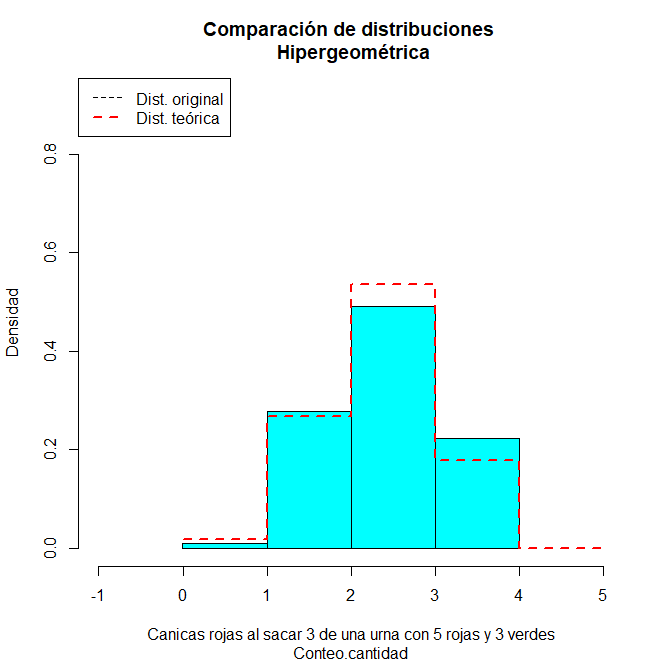
\includegraphics[scale=0.35]{Problema_84.png}
 \end{center}
 El cual coincide con los datos obtenidos,
 que es a lo que se quer\'{\i}a llegar.${}_{\blacksquare}$
\end{solucion}
